%%
%% Author: Fabian Klopfer (fabian.klopfer@ieee.org) 
%%

% Preamble
\documentclass[a4paper]{article}

% Packages
\usepackage[utf8]{inputenc}
\usepackage[T1]{fontenc}
\usepackage{enumerate}
\usepackage{fancyhdr}
\usepackage{amssymb}
\usepackage{amsmath}
\usepackage{amsfonts}
\usepackage{a4wide}
\usepackage{graphicx}
\usepackage{wrapfig}
\usepackage{tikz}
\usepackage{listings}
\usepackage{colortbl}
\usepackage{tabularx}
\usepackage{hyperref}
\usepackage{multicol}
\usepackage{float}

\setlength{\headheight}{24pt}

\pagestyle{fancy}
\lhead{Custom Sample Exam 0}
\rhead{Compiler Construction}

% Variables to generate:
% Ex. 1: Automaton, RegEx (both https://cyberzhg.github.io/toolbox/) (ba*(ϵ|a)*acb*|ϵ), 
% Ex. 2: Grammar, LL(1) (https://cyberzhg.github.io/toolbox/)
% Ex. 3: Code for IR, Graph (loops, ifs, array, arith.; fixed list)
% Ex. 4: AST, Code control flow (use oberon0c, use method from above)
% Ex. 5: ASM code for sched, which scheduling to use (use oberon0c, fixed list)
% Ex. 6: ASM code for alloc., which algos to use 1,2 (use oberon0c, fixed list) P. 644


% Document
\begin{document}
	\section*{Exercise 1: Scanners}\label{sec:exercise1}
   \begin{enumerate}[a.]
		\item Describe informally the language the automaton accepts \\
		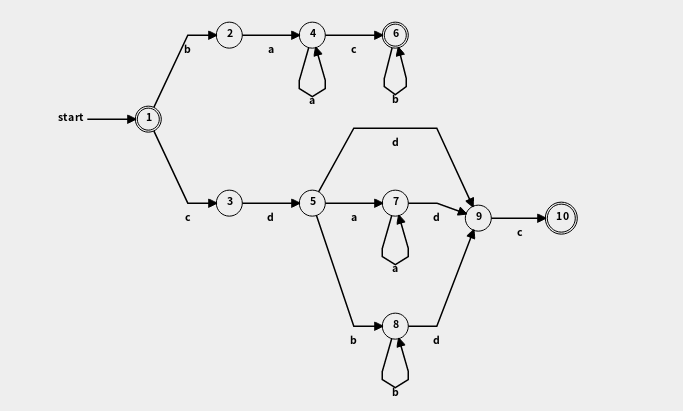
\includegraphics[keepaspectratio,width=0.4\textwidth]{exam_img/automaton_0}
        \item Do Thompsons construction, subset construction, Hopcroft minimization on the reg ex $(a|b)*cb(a*b*|\varepsilon)$
   \end{enumerate}

	\section*{Exercise 2: Parsers}\label{sec:exercise2}
        \begin{enumerate}[a.]
            \item write a context-free grammar for Boolean expressions
            \item Use the just contructed grammar. Is it LL(1), if not so make it LL(1). \\
           
        \end{enumerate}


	\section*{Exercise 3: IR}\label{sec:exercise3}
	\begin{lstlisting}
int[] a = {0,0,0,0,0};
int c = 1;
for (i=0; i < 20; ++i) {
  if (a[4] = 1) {
    c++;
  } else {
    a[i] = c;
  }
}
if (c == 2)
  while (true) {
    c++;
    if (c > 999) {
	  break;
	}
  }
} else if (c == 1 ) {
  a[i] = 3;
}	
	\end{lstlisting}
	\begin{enumerate}[a.]
        \item sketch an @GRAPH
        \item for what applications can @GRAPH be used
    \end{enumerate}
\newpage
	\section*{Exercise 4: Code Shape}\label{sec:exercise4}
	\begin{lstlisting}
statement_sequence
|-assignment
|-|-ADDR x: Type as Variable | Offset: 0
|-|-CONSTANT const0: Constant as Variable | Value: 10
|-assignment
|-|-ADDR y: Type as Variable | Offset: 4
|-|-CONSTANT const1: Constant as Variable | Value: 3
|-assignment
|-|-ADDR z: Type as Variable | Offset: 8
|-|-DIV
|-|-|-DEREF x: Type as Variable | Offset: 0
|-|-|-+
|-|-|-|-DEREF y: Type as Variable | Offset: 4
|-|-|-|-CONSTANT const2: Constant as Variable | Value: 1
|-assignment
|-|-ADDR x: Type as Variable | Offset: 0
|-|-*
|-|-|--
|-|-|-|-*
|-|-|-|-|-CONSTANT Pi: Constant as Variable | Value: 3
|-|-|-|-|-DEREF z: Type as Variable | Offset: 8
|-|-|-|-DEREF y: Type as Variable | Offset: 4
|-|-|--
|-|-|-|-*
|-|-|-|-|-CONSTANT Pi: Constant as Variable | Value: 3
|-|-|-|-|-DEREF z: Type as Variable | Offset: 8
|-|-|-|-DEREF y: Type as Variable | Offset: 4
|-assignment
|-|-ADDR y: Type as Variable | Offset: 4
|-|-*
|-|-|-DEREF x: Type as Variable | Offset: 0
|-|-|-DIV
|-|-|-|-CONSTANT const3: Constant as Variable | Value: 1
|-|-|-|-DEREF z: Type as Variable | Offset: 8

	\end{lstlisting}
\begin{enumerate}[a.]
	\item use treewalk code gen assuming unlimited registers
	\item Sketch the control flow of the following code snippets \\
	\newpage
		\begin{lstlisting}
int[] a = {0,0,0,0,0};
int c = 1;
for (i=0; i < 20; ++i) {
  if (a[4] = 1) {
    c++;
  } else {
    a[i] = c;
	if (c == 2){
	  while (true) {
	    c++;
		if (c > 999) {
		  break;
		}
	  }
	} else if (c == 1 ) {
	  a[i] = 3;
	}	
  }
}
if (c == 2)
  while (true) {
    c++;
	if (c > 999) {
	  break;
	}
  }
} else if (c == 1 ) {
  a[i] = 3;
}	
	\end{lstlisting}
\end{enumerate}

	\section*{Exercise 5: Instruction Selection \& Scheduling}\label{sec:exercise5} 
	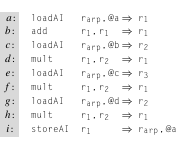
\includegraphics[keepaspectratio,width=0.4\textwidth]{exam_img/iloc_0_0}
\begin{enumerate}[a.]
	\item draw the dependence graph and annotate each node with the cummulative latency
	\item use global list scheduling to schedule the code fragment
\end{enumerate}

	\section*{Exercise 6: Register Allocation}\label{sec:exercise6}
	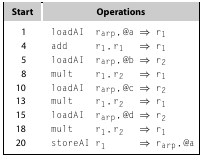
\includegraphics[keepaspectratio,width=0.4\textwidth]{exam_img/iloc_0_1}
\begin{enumerate}[a.]
	\item write down the live ranges as set of intervals
	\item show the result of using the bottom-up global algorithm on it to alloc registers
	\item show the result of using the top-down global algorithm on it to alloc registers
\end{enumerate}
\end{document}
